\chapter{Extracting and Analyzing Results}

\glc\ stores its output in an \href{http://www.hdfgroup.org/HDF5/}{HDF5} file. The contents of this file can be viewed and manipulated using a variety of ways including:
\begin{description}
 \item[\href{http://www.hdfgroup.org/hdf-java-html/hdfview/}{{\sc HDFView}}] This is a graphical viewer for exploring the contents of HDF5 files;
 \item[\href{http://www.hdfgroup.org/products/hdf5_tools/index.html\#h5dist}{HDF5 Command Line Tools}] A set of tools which can be used to extract data from HDF5 files (\href{http://www.hdfgroup.org/HDF5/doc/RM/Tools.html#Tools-Dump}{{\tt h5dump}} and \href{http://www.hdfgroup.org/HDF5/doc/RM/Tools.html#Tools-Ls}{{\tt h5ls}} are particularly useful);
 \item[\href{http://www.hdfgroup.org/HDF5/doc/RM/RM_H5Front.html\#F90andCPPlus}{C++ and Fortran 90 APIs}] Allow access to and manipulation of data in HDF5 files;
 \item[\href{http://code.google.com/p/h5py/}{{\sc h5py}}] A Python interface to HDF5 files.
\end{description}

In the remainder of this section the structure of \glc\ HDF5 files is described and a general-purpose Perl module which we use to extract data in a convenient manner is outlined.

\section{General Structure of Output File}

Figure~\ref{fig:glcOutputFileStructure} shows the structure of a typical \glc\ output file. The various groups and subgroups are described below.

\begin{figure}
\begin{center}
\begin{verbatim}
outputFile.hdf5
 |
 +-> UUID                                     Attribute {1}
 |
 +-> Build                                    Group
 |    |
 |    +-> FGSL_library_version                Attribute {1}
 |    +-> FoX_library_version                 Attribute {1}
 |    +-> GSL_library_version                 Attribute {1}
 |    +-> HDF5_library_version                Attribute {1}
 |    +-> make_CCOMPILER                      Attribute {1}
 |    +-> make_CCOMPILER_VERSION              Attribute {1}
 |    +-> make_CFLAGS                         Attribute {1}
 |    +-> make_CPPCOMPILER                    Attribute {1}
 |    +-> make_CPPCOMPILER_VERSION            Attribute {1}
 |    +-> make_CPPFLAGS                       Attribute {1}
 |    +-> make_FCCOMPILER                     Attribute {1}
 |    +-> make_FCCOMPILER_VERSION             Attribute {1}
 |    +-> make_FCFLAGS                        Attribute {1}
 |    +-> make_FCFLAGS_NOOPT                  Attribute {1}
 |    +-> make_MODULETYPE                     Attribute {1}
 |    +-> make_PREPROCESSOR                   Attribute {1}
 |    +-> sourceChangeSetDiff                 Dataset   {1}
 |    +-> sourceChangeSetMerge                Dataset   {1}
 |
 +-> Outputs                                  Group
 |    |
 |    +-> Output1                             Group
 |    |    |
 |    |    +-> nodeData                       Group
 |    |    |     |
 |    |    |     +-> nodeProperty1            Dataset {<nodeCount>}
 |    |    |     +-> ...                      Dataset {<nodeCount>}
 |    |    |     +-> ...                      Dataset {<nodeCount>}
 |    |    |     +-> ...                      Dataset {<nodeCount>}
 |    |    |     +-> nodePropertyN            Dataset {<nodeCount>}
 |    |    |
 |    |    +-> mergerTreeCount                Dataset {<treeCount>}
 |    |    |
 |    |    +-> mergerTreeIndex                Dataset {<treeCount>}
 |    |    |
 |    |    +-> mergerTreeStartIndex           Dataset {<treeCount>}
 |    |    |
 |    |    +-> mergerTreeWeight               Dataset {<treeCount>}
 |    |    |
 |    |    +-> mergerTree1                    Group              [optional]
 |    |    |     |
 |    |    |     +-> nodeProperty1            Reference
 |    |    |     +-> ...                      Reference
 |    |    |     +-> ...                      Reference
 |    |    |     +-> ...                      Reference
 |    |    |     +-> nodePropertyN            Reference
 |    |    |
 |    |    x-> ...                            Group              [optional]
 |    |    x-> ...                            Group              [optional]
 |    |    x-> ...                            Group              [optional]
 |    |    x-> mergerTree<treeCount>          Group              [optional]
 |    |    |
 |    |    +-> outputExpansionFactor          Attribute {1}
 |    |    +-> outputTime                     Attribute {1}
 |    |
 |    x-> Output2                             Group
 |
 +-> Parameters                               Group
 |    |
 |    +-> inputParameter1                     Attribute {}
 |    +-> ...                                 Attribute {}
 |    +-> ...                                 Attribute {}
 |    +-> ...                                 Attribute {}
 |    +-> inputParameterN                     Attribute {}
 |
 +-> Version                                  Group
 |    |
 |    +-> runTime                             Attribute {1}
 |    +-> versionMajor                        Attribute {1}
 |    +-> versionMinor                        Attribute {1}
 |    +-> versionRevision                     Attribute {1}
 |    +-> hgRevision                          Attribute {1}
 |    +-> hgHash                              Attribute {1}
 |    +-> runByName                           Attribute {1}
 |    +-> runByEmail                          Attribute {1}
 |
 +-> globalHistory                            Group
      |
      +-> historyExpansion                    Dataset {<historyCount>}
      +-> historyStarFormationRate            Dataset {<historyCount>}
      +-> historyTime                         Dataset {<historyCount>}
\end{verbatim}
\end{center}
\caption{Structure of a \glc\ HDF5 output file. {\tt <treeCount>} is the total number of merger trees present in a given output, and {\tt <nodeCount} is the total number of nodes (in all trees) present in an output.}
\label{fig:glcOutputFileStructure}
\end{figure}

\subsection{UUID}\label{sec:UUID}

The UUID (\href{https://secure.wikimedia.org/wikipedia/en/wiki/Universally_unique_identifier}{Universally Unique Identifier}) is a unique identifier assigned to each \glc\ model that is run. It allows identification of a given model and can be referenced from, for example, an external database. Using the {\tt Galacticus::HDF5} Perl module (see \S\ref{sec:perlModuleDataExtraction}), the UUID can be loaded into the data structure using:
\begin{verbatim}
&HDF5::Get_UUID($model);
\end{verbatim}
The UUID is then available as {\tt \$model-\textgreater\{'uuid'\}}.

\subsection{Build Information}\label{sec:BuildInformation}

\glc\ automatically stores various information about how it was built in the {\tt Build} group attributes. Currently, included attributes consist of:
\begin{description}
\item[{\tt FGSL\_library\_version}] The version number of the FGSL library;
\item[{\tt FoX\_library\_version}] The version number of the FoX library;
\item[{\tt GSL\_library\_version}] The version number of the GSL library;
\item[{\tt HDF5\_library\_version}] The version number of the HDF5 library;
\item[{\tt make\_CCOMPILER}] The C compiler command used;
\item[{\tt make\_CCOMPILER\_VERSION}] The C compiler version information;
\item[{\tt make\_CFLAGS}] The flags passed to the C compiler;
\item[{\tt make\_CPPCOMPILER}] The C++ compiler command used;
\item[{\tt make\_CPPCOMPILER\_VERSION}] The C++ compiler version information;
\item[{\tt make\_CPPFLAGS}] The flags passed to the C++ compiler;
\item[{\tt make\_FCCOMPILER}] The Fortran compiler command used;
\item[{\tt make\_FCCOMPILER\_VERSION}] The Fortran compiler version information;
\item[{\tt make\_FCFLAGS}] The flags passed to the Fortran compiler;
\item[{\tt make\_FCFLAGS\_NOOPT}] The flags passed to the Fortran compiler for unoptimized compiles;
\item[{\tt make\_MODULETYPE}] The Fortran module type identifier string;
\item[{\tt make\_PREPROCESSOR}] The preprocessor command used.
\end{description}

Additionally, two datasets are included which store details of the \glc\ source changeset. {\tt sourceChangeSetMerge} contains the output of ``{\tt hg bundle -t none}'', that is, it contains a Mercurial changegroup that incorporates any changes made to the current branch relative to the main \glc\ branch. {\tt sourceChangeSetDiff} contains the output of ``{\tt hg diff}'', that is, all differences between the source code in the working directory and that which has been committed to Mercurial. Used together, these two datasets allow the precise source code used to run the model to be recovered from the main branch \glc\ source.

\subsection{Parameters}

The {\tt Parameters} group contains a record of all parameter values (either input or default) that were used for this \glc\ run. The group contains a long list of attributes, each attribute named for the corresponding parameter and with a single entry giving the value of that parameter. The {\tt scripts/aux/Extract\_Parameter\_File.pl} script can be used to extract these parameter values to an XML file suitable for re-input into \glc.

\subsection{Version}

The {\tt Version} group contains a record of the \glc\ version used for this model, storing the major and minor version numbers, the revision number and the {\sc Mercurial} revision and hash (if the code is being maintained using {\sc Mercurial}, otherwise a value of $-1$ is entered or the revision and the hash attribute is empty). Additionally, the time at which the model was run is stored and, if the {\tt galacticusConfig.xml} file (see \S\ref{sec:ConfigFile}) is present and contains contact details, the name and e-mail address of the person who ran the model.

\subsection{globalHistory}\label{sec:globalHistory}\index{history!global}\index{outputs!global history}

The {\tt globalHistory} group stores volume averaged properties of the model universe as a function of time. Currently, the properties stored are:
\begin{description}
 \item[{\tt historyTime}] Cosmic time (in Gyr);
 \item[{\tt historyExpansion}] Expansion factor;
 \item[{\tt historyStarFormationRate}] Volume averaged star formation rate (in $M_\odot/$Gyr/Mpc$^3$).
 \item[{\tt historyDiskStarFormationRate}] Volume averaged star formation rate in disks (in $M_\odot/$Gyr/Mpc$^3$).
 \item[{\tt historySpheroidStarFormationRate}] Volume averaged star formation rate in spheroids (in $M_\odot/$Gyr/Mpc$^3$).
 \item[{\tt historyStellarDensity}] Volume averaged stellar mass density (in $M_\odot/$Mpc$^3$).
 \item[{\tt historyDiskStellarDensity}] Volume averaged stellar mass density in disks (in $M_\odot/$Mpc$^3$).
 \item[{\tt historySpheroidStellarDensity}] Volume averaged stellar mass density in spheroids (in $M_\odot/$Mpc$^3$).
 \item[{\tt historyGasDensity}] Volume averaged cooled gas density (in $M_\odot/$Mpc$^3$).
 \item[{\tt historyNodeDensity}] Volume averaged resolved node density (in $M_\odot/$Mpc$^3$).
\end{description}
Dimensionful datasets have a {\tt unitsInSI} attribute which gives their units\index{units} in the SI system.

\subsection{Outputs}

The {\tt Outputs} group contains one or more sub-groups corresponding to the output times requested from \glc. Each sub-group contains the following information:
\begin{description}
 \item[{\tt outputTime} \emph{(attribute)}] The cosmic time (in Gyr) at this output;
 \item[{\tt outputExpansionFactor} \emph{(attribute)}] The expansion factor at this output;
 \item[{\tt nodeData}] A group of node properties as described below.
 \item[{\tt mergerTree} subgroups \emph{(optional)}] A set of {\tt mergerTree} groups as described below.
\end{description}

\subsubsection{nodeData group}\label{sec:nodeDataGroup}

The {\tt nodeData} group contains all data from nodes in all merger trees. The group consists of a collection of datasets each of which lists a property of all nodes in the trees which exist at the output time. Where relevant, each dataset contains an attribute, {\tt unitsInSI}, which gives the units\index{units} of the dataset in the SI system.

\subsubsection{mergerTree datasets}\label{sec:mergerTreeDatasets}

To allow locating of nodes belonging to a given merger tree in the datasets in the {\tt nodeData} group, the {\tt mergerTreeStartIndex} and {\tt mergerTreeCount} datasets list the starting index of each tree's nodes in the {\tt nodeData} datasets, and the number of nodes belonging to each tree respectively. Additionally, the {\tt mergerTreeWeight} dataset lists the {\tt volumeWeight} property for each tree (see \S\ref{sec:mergerTreeSubgroups}) which gives the weight (in Mpc$^{-3}$) which should be assigned to this tree (and all nodes in it) to create a volume-averaged sample (see \S\ref{sec:volumeLimitedSamples}). Finally, the {\tt mergerTreeIndex} dataset gives the index of each tree stored in the {\tt nodeData} datasets.

\subsubsection{mergerTree subgroups}\label{sec:mergerTreeSubgroups}

These subgroups will be present if the {\tt [mergerTreeOutputReferences]} parameter is set to true. Each {\tt mergerTree} subgroup contains HDF5 references to all data on a single merger tree. The group consists of a collection of scalar references each of which points to the appropriate region of the corresponding dataset in the {\tt nodeData} group. Additionally, the {\tt volumeWeight} attribute of this group gives the weight (in Mpc$^{-3}$) which should be assigned to this tree (and all nodes in it) to create a volume-averaged sample. (A second attribute, {\tt volumeWeightUnitsInSI}, gives the units of {\tt volumeWeight} in the SI system.)

\subsection{Optional Outputs}

Numerous other quantities can be optionally output. These are documented below:

\subsubsection{Redshifts}\index{redshift!output}\index{output!redshift}

The redshift corresponding to the time at which a node was last isolated can be output by setting {\tt [outputNodeRedshifts]} to {\tt true}. This quantity will be output as {\tt basicRedshiftLastIsolated}.

\subsubsection{Mass Accretion Histories}

A mass accretion history (i.e. mass as a function of time) for the main branch in each merger tree can be output by setting {\tt massAccretionHistoryOutput}$=${\tt true}. If requested, a new group {\tt massAccretionHistories} will be made in the \glc\ output file. It will contain groups called {\tt mergerTreeN} where {\tt N} is the merger tree index. Each such group will contain the following three datasets, defined for the main branch of the tree\footnote{``Main branch'' is defined by starting from the root node of a tree and repeatedly stepping back to the most massive progenitor of the branch. This does not necessarily pick out the most massive progenitor at a given time.}:
\begin{description}
 \item [{\tt nodeIndex}] The index of the node in the tree;
 \item [{\tt nodeTime}] The time at this point in the tree (in Gyr);
 \item [{\tt nodeMass}] The mass of the node at this point in the tree (in $M_\odot$). The {\tt nodeMass} property is defined to be the total mass of each node in a merger tree. Therefore, it includes both dark and baryonic mass. Additionally, the mass of a node includes the mass of any satellite nodes that it may contain. The mean density of the node depends on the method selected by the {\tt virialDensityContrastMethod} parameter.
\end{description}

\subsubsection{Merger Tree Dump}

A full dump of merger tree structure by setting {\tt mergerTreeStructureDump}$=${\tt true}. In this case, files will be dumped to the directory specified by {\tt [mergerTreeStructureDumpDirectory]} for each merger tree with final mass between {\tt [mergerTreeStructureDumpMassMinimum]} and {\tt [mergerTreeStructureDumpMassMaximum]}. Each tree is dumped to a file named ``{\tt mergerTreeDump:\textless treeIndex\textgreater:1.gv}'' in the specified directory in {\sc GraphViz} format.

\subsubsection{Conditional Mass Functions}

Setting {\tt [mergerTreeComputeConditionalMassFunction]}$=${\tt true} will cause conditional mass functions to be computed and output to the \glc\ output file in a group named ``{\tt conditionalMassFunction}''. The mass functions are binned in parent halo mass, and the mass ratio of the progenitor to parent halo. Bins are logarithmically spaced in mass (and mass ratio), with the range and number of bins controlled by the parameters:
\begin{itemize}
\item {\tt [mergerTreeComputeConditionalMassFunctionParentMassCount]};
\item {\tt [mergerTreeComputeConditionalMassFunctionParentMassMinimum]};
\item {\tt [mergerTreeComputeConditionalMassFunctionParentMassMaximum]};
\item {\tt [mergerTreeComputeConditionalMassFunctionMassRatioCount]};
\item {\tt [mergerTreeComputeConditionalMassFunctionMassRatioMinimum]};
\item {\tt [mergerTreeComputeConditionalMassFunctionMassRatioMaximum]}.
\end{itemize}
The resulting parent masses and mass ratios are written to datasets {\tt massParent} and {\tt massRatio} respectively. Parent and progenitor halos are defined at a set of redshifts defined by the arrays {\tt [mergerTreeComputeConditionalMassFunctionParentRedshifts]}, and {\tt [mergerTreeComputeConditionalMassFunctionProgenitorRedshifts]}, which are written to datasets {\tt redshiftParent} and {\tt redshiftProgenitor}. The resulting conditional masses functions are written to datasets {\tt conditionalMassFunction} and {\tt conditionalMassFunctionError}.

In addition to standard progenitor mass functions, the progenitor mass function conditioned on progenitor rank (i.e. 1$^{\rm st}$ most massive, 2$^{\rm nd}$, \ldots, $n^{\rm th}$ most massive progenitor) is computed and output to the datasets {\tt primaryProgenitorMassFunction} and {\tt primaryProgenitorMassFunctionError}. The depth (i.e. $n$) is specifed by {\tt [mergerTreeComputeConditionalMassFunctionPrimaryProgenitorDepth]}.

Finally, the progenitor mass functoin conditioned on recent formation is computed and output to the datasets {\tt formationRateFunction} and {\tt formationRateFunctionError}. To be considered ``recently formed'' a progenitor must have formed between $t$ and $t(1-\Delta)$ where $t$ is the progenitor time and $\Delta=${\tt [mergerTreeConditionalMassFunctionFormationRateTimeFraction]}.

\subsubsection{Pre-Evolution Merger Trees}

\glc\ can output the full structure of merger trees prior to any evolution. Merger tree structure can be requested by setting {\tt mergerTreeStructureOutput}$=${\tt true}. Structures are written to a new group, {\tt mergerTreeStructures}, in the \glc\ output file. This group will contain groups called {\tt mergerTreeN} where {\tt N} is the merger tree index. Each such group will contain the following datasets:
\begin{description}
 \item [{\tt nodeIndex}] The index of the node in the tree;
 \item [{\tt childIndex}] The index of this node's first child node;
 \item [{\tt parentIndex}] The index of this node's parent node;
 \item [{\tt siblingIndex}] The index of this node's sibling node;
 \item [{\tt nodeTime}] The time at this point in the tree (in Gyr);
 \item [{\tt nodeMass}] The mass of the node at this point in the tree (in $M_\odot$). The {\tt nodeMass} property is defined to be the total mass of each node in a merger tree. Therefore, it includes both dark and baryonic mass. Additionally, the mass of a node includes the mass of any satellite nodes that it may contain. The mean density of the node depends on the method selected by the {\tt virialDensityContrastMethod} parameter.
\end{description}
Additional, optional, datasets can be added by setting appropriate input parameters. Currently these include:
\begin{itemize}
 \item [Virial quantities] If {\tt mergerTreeStructureOutputVirialQuantities}$=${\tt true} then two additional datasets are included:
 \begin{description}
  \item [{\tt nodeVirialRadius}] The virial radius of the node (in Mpc);
  \item [{\tt nodeVirialVelocity}] The virial velocity of the node (in km/s);
 \end{description}
 \item [Dark matter scale radii] If {\tt mergerTreeStructureOutputDarkMatterScaleRadius}$=${\tt true} then an additional dataset is included:
 \begin{description}
  \item [{\tt darkMatterScaleRadius}] The scale radius of this node's dark matter halo profile (in Mpc);
 \end{description}
 \item [Merger tree final descendent] If {\tt outputFinalDescendentIndices}$=${\tt true} then an additional dataset is included:
 \begin{description}
  \item [{\tt finalDescendentIndex}] The index of the final descendent that this node will reach in its merger trees;
 \end{description}
\end{itemize}

\section{Perl Module for Data Extraction}\label{sec:perlModuleDataExtraction}

A Perl module is provided that allows for easy extraction of datasets from the \glc\ output file together with a straightforward way to implement derived properties. To use this Perl module, add
\begin{verbatim}
 use lib "./perl";
 use PDL;
 use Galacticus::HDF5;
\end{verbatim}
at the start of your Perl script. The {\tt Galacticus::HDF5} module will import data from a \glc\ HDF5 file into PDL variables. All data are stored in a single structure, which also specifies the file, output and range of trees to read. An example of reading a dataset from a file is:
\begin{verbatim}
 my $model;
 $model->{'file'     } = "galacticus.hdf5";
 $model->{'output'   } = 1;
 $model->{'tree'     } = "all";
 $model->{'dataRange'} = [1,2];
 $model->{'store'    } = 0;
 &HDF5::Get_Dataset($model,['nodeMass']);
 $dataSets = $model->{'dataSets'};
 print $dataSets->{'nodeMass'}."\n";
\end{verbatim}
The {\tt \$model} object is initialized with information to specify which file, output and trees should be used. Its settable components are:
\begin{description}
 \item [{\tt file}] The name of the \glc\ output file to be read.
 \item [{\tt output}] Specify the output number in the file which should be read.
 \item [{\tt tree}] Specify the tree which should be read, or use ``all'' to specify that all trees be read.
 \item [{\tt dataRange}] Gives the first and last entry in the dataset to read---this facilitates reading of partial datasets (and therefore reading datasets in a piecemeal fashion). If this component is missing, the entire dataset is read.
 \item[{\tt store}] If set to 1, any derived properties will be stored back in the \glc\ output file for later retrieval. If set to 0 (or if this option is not present), derived properties will not be stored. Currently, storing of derived properties in the \glc\ file is only possible if the {\tt tree} option is set to ``all'' and no {\tt dataRange} is specified.
\end{description}
The {\tt \&HDF5::Get\_Dataset(\$model,['nodeMass']);} call requests that the {\tt nodeMass} dataset be read. It is return as a PDL variable in the {\tt nodeMass} element of the {\tt dataSets} element which is itself a member of {\tt \$model}. The final lines in the example simply write out the resulting array of {\tt nodeMass} values.

\subsection{Derived Properties}

Derived properties can be created by giving defining functions along with a regular expression string that allows them to be matched. For example, the {\tt Galacticus::Baryons} module implements a hot gas fraction property called {\tt hotHaloFraction} or {\tt hotHaloFrac}. It has the following form:
\begin{verbatim}
package Baryons;
use PDL;
use Galacticus::HDF5;
use Data::Dumper;

%HDF5::galacticusFunctions = ( %HDF5::galacticusFunctions,
    "hotHalo(Fraction|Frac)" => \&Baryons::Get_hotHaloFraction
    );

my $status = 1;
$status;

sub Get_hotHaloFraction {
    $model = shift;
    $dataSetName = $_[0];
    &HDF5::Get_Dataset($model,['hotHaloMass','nodeMass']);
    $dataSets = $model->{'dataSets'};
    $dataSets->{$dataSetName} = $dataSets->{'hotHaloMass'}/$dataSets->{'nodeMass'};
}

\end{verbatim}
The module begins by adding an entry to the {\tt \%HDF5::galacticusFunctions} hash. The key gives a regular expression which matches to the name of the property to be defined. The value of the key gives a reference to a subroutine to be called to evaluate this expression. The subroutine is defined below. When called, it receives the {\tt \$model} structure along with the name of the requested property. The subroutine should then simply evaluate the requested property and store it in the appropriate location within {\tt \$model}. Note that the subroutine can request additional datasets be loaded (as happens above where {\tt hotHaloMass} and {\tt nodeMass} are requested) if they are needed for its calculations.

\subsubsection{Available Derived Properties}\label{sec:DerivedProperties}

\begin{description}
 \item[{\tt mergerTreeIndex}] The index of the merger tree in which the galaxy is found. Provided by: {\tt Galacticus::HDF5}.
 \item[{\tt redshift}] The redshift at which the galaxy exists. Provided by: {\tt Galacticus::Time}.
 \item[{\tt time}] The cosmic time (in Gyr) at which the galaxy exists. Provided by: {\tt Galacticus::Time}.
 \item[{\tt expansionFactor}] The expansion factor at which the galaxy exists. Provided by: {\tt Galacticus::Time}.
 \item[{\tt stellarMass}] The sum of disk and spheroid stellar masses. Provided by: {\tt Galacticus::StellarMass}.
 \item[{\tt massColdGas}] The sum of disk and spheroid cold gas masses. Provided by: {\tt Galacticus::GasMass}.
 \item[{\tt starFormationRate}] The sum of disk and spheroid star formation rates. Provided by: {\tt Galacticus::StellarMass}.
 \item[{\tt hostNodeMass}] For isolated nodes, the node mass. For non-isolated nodes, the mass of the isolated node in which the node resides. Provided by: {\tt Galacticus::HostNode}.\index{nodes!host mass}\index{halos!host mass}\index{satellites!host mass}
 \item[{\tt stellarMass}] The sum of disk and speheroid stellar masses (or, whichever of these exist in the model). Provided by: {\tt Galacticus::StellarMass}.
 \item[{\tt hotHalo(Fraction\textbar Frac)}] The fraction the node's mass in the hot gas halo. Provided by: {\tt Galacticus::Baryons}.
 \item[{\tt inclination}] A randomly selected inclination for the disk (in degrees). Provided by: {\tt Galacticus::Inclination}.
 \item[{\tt \textasciicircum(disk\textbar bulge)StellarLuminosity:.*:dustAtlas($\backslash$[faceOn$\backslash$])\$}] Dust-extingiushed\index{dust!extinction} luminosities for disk and bulge found by interpolating in the dust tables of \cite{ferrara_atlas_1999}. If the {\tt [faceOn]} qualifier is present, extinctions are computed assuming that the disk is observed face-on, otherwise a random inclination is used. Optionally, the dust atlas file to used can be specified via {\tt \$dataSet-\textgreater\{'dustAtlasFile'\}}. The available dust atlases span a limited range of spheroid sizes and central optical depths in their tabulations. Standard behavior is to extrapolate beyond the ends of these ranges. This can be controlled via {\tt \$dataSet-\textgreater\{'dustAtlasExtrapolateInSize'\}} and {\tt \$dataSet-\textgreater\{'dustAtlasExtrapolateInTau'\}} respectively, which can be set to {\tt yes}/{\tt no} (or, equivalently, 1/0). Provided by: {\tt Galacticus::DustAttenuation}.
 \item[{\tt \textasciicircum(disk\textbar bulge)LuminositiesStellar:.*:dustCharlotFall2000\$}] Dust-extingiushed\index{dust!extinction} luminosities for disk and bulge found using the model of \cite{charlot_simple_2000}. Provided by: {\tt Galacticus::DustCharlotFall2000}.
 \item[{\tt \textasciicircum totalStellarLuminosity:.*:dustAtlas($\backslash$[faceOn$\backslash$])\$}] (Optionally dust-extingiushed) luminosities for disk plus bulge found by adding together the corresponding disk and bulge luminosities. Provided by: {\tt Galacticus::Luminosities}.
 \item[{\tt \textasciicircum bulgeToTotalLuminosity:.*:dustAtlas($\backslash$[faceOn$\backslash$])\$}] Ratio of bulge to total (optionally dust-extingiushed) luminosities. Provided by: {\tt Galacticus::Luminosities}.
 \item[{\tt \textasciicircum magnitude([\textasciicircum :]+):([\textasciicircum :]+):([\textasciicircum :]+):z([$\backslash$d$\backslash$.]+)(:dust[\textasciicircum :]+)?(:vega\textbar :AB)?}] Absolute magnitude corresponding to a stellar luminosity, in either Vega or AB systems. Provided by: {\tt Galacticus::Magnitudes}.
 \item[{\tt \textasciicircum magnitude:(.*)(:vega\textbar :AB)?}] Absolute magnitude corresponding to the generic luminosity property {\tt \textasciicircum luminosity:\$1}, in either Vega or AB systems. Provided by: {\tt Galacticus::Magnitudes}.
 \item[{\tt \textasciicircum apparentMagnitude:(.*)}] Apparent magnitude corresponding to the absolute magnitude {\tt \textasciicircum magnitude:\$1}. Provided by: {\tt Galacticus::Magnitudes}.
 \item[{\tt comovingDistance}] The comoving distance (in Mpc) to the galaxy---provided by {\tt Galacticus::Survey} (see \S\ref{sec:Galacticus::Survey} for a full description).
 \item[{\tt luminosityDistance}] The luminosity distance (in Mpc) to the galaxy---provided by {\tt Galacticus::Survey} (see \S\ref{sec:Galacticus::Survey} for a full description).
 \item[{\tt distanceModulus}] The distance modulus (including the $+2.5\log_{10}(1+z)$ term to account for squeezing of photon frequencies) to the galaxy---provided by {\tt Galacticus::Survey} (see \S\ref{sec:Galacticus::Survey} for a full description).
 \item[{\tt redshift}] The redshift at which the galaxy is observed---provided by {\tt Galacticus::Survey} (see \S\ref{sec:Galacticus::Survey} for a full description).
 \item[{\tt angularWeight}] The weight (in units of ) which should be assigned to this galaxy in order to build a redshift survey---provided by {\tt Galacticus::Survey} (see \S\ref{sec:Galacticus::Survey} for a full description).
 \item[{\tt angularDiameterDistance}] The angular diameterer distance (in Mpc) to the galaxy---provided by {\tt Galacticus::Survey} (see \S\ref{sec:Galacticus::Survey} for a full description).
 \item[{\tt \textasciicircum angularPosition[12]}] The angular position (in radians measured along two orthogonal axes from the center of the field) of the galaxy---provided by {\tt Galacticus::Survey} (see \S\ref{sec:Galacticus::Survey} for a full description).
 \item[{\tt \textasciicircum grasilFlux[$\backslash$d$\backslash$.]+microns}] The flux at the given wavelength (specific in microns) of the galaxy as computed by the {\tt Grasil} code (see \S\ref{sec:Grasil} for a full description).
 \item[{\tt \textasciicircum grasilInfraredLuminosity}] The total infrared (8--1000$\mu$m) luminosity of the galaxy as computed by the {\tt Grasil} code (see \S\ref{sec:Grasil} for a full description).
 \item[{\tt \textasciicircum grasilFlux:([\textasciicircum :]+)}] The flux (in Janskys) of the galaxy as computed by the {\tt Grasil} code integrated under the specified filter (see \S\ref{sec:Grasil} for a full description).
 \item[{\tt \textasciicircum luminosity:grasil:([\textasciicircum :]+):([\textasciicircum :]+)}] The luminosity (in units of the zero point of the AB magnitude system) of the galaxy as computed by the {\tt Grasil} code integrated under the specified filter and in the specified frame (see \S\ref{sec:Grasil} for a full description).
 \item[{\tt flux850micronHayward}] The flux of the galaxy at 850$\mu$m\index{flux!sub-mm} computed using the fitting formula of \cite{hayward_what_2010}, specifically:
\begin{equation}
 {S_{850\mu{\rm m}} \over {\rm Jy}} = A \left({\dot{M}_\star \over 100 M_\odot \hbox{Gyr}^{-1}}\right)^\alpha \left({R_{\rm dust} M_{\rm metals,gas} \over 10^8 M_\odot}\right)^\beta,
\end{equation}
where $R_{\rm dust}$ is the dust-to-metals ratio, $\dot{M}_\star$ is the total star formation rate in the galaxy and $M_{\rm metals,gas}$ is the total mass of metals in the gas phase of the galaxy. Note that the fit given by \cite{hayward_what_2010} was computed for galaxcy at $z\approx 2$. The parameters of the fit can be specified by setting elements of {\tt \$model-\textgreater\{'haywardSubMmFit'\}}: {\tt \{'dustToMetalsRatio'\}}$\equiv R_{\rm dust}$, {\tt \{'fitNormalization'\}}$\equiv A$, {\tt \{'starFormationRateExponent'\}}$\equiv \alpha$, and {\tt \{'dustMassExponent'\}}$\equiv \beta$. If these elements are not present the default values of $A=0.65\times 10^{-3}$, $R_{\rm dust}=0.61$, $\alpha=0.42$ and $\beta = 0.58$ \cite{hayward_what_2010} will be used instead. Provided by: {\tt Galacticus::SubMmFluxesHayward}.
 \item[{\tt \textasciicircum(disk|spheroid|total)LymanContinuumLuminosity:z[$\backslash$d$\backslash$.]+\$}] The luminosity (in units of $10^{50}$photons/s) of the \gls{LymanContinuum} radiation of the disk or spheroid component, or total of the two at the specified redshift. The rest-frame {\tt Lyc} filter must have been computed in \glc\ to allow this luminosity to be computed. If the {\tt Lyc} filter was computed with a non-default postprocessing chain then the name of the chain should be specified in {\tt \$dataBlock-\textgreater\{'lymanContinuum'\}-\textgreater\{'postProcessingChain'\}} Provided by: {\tt Galacticus::Lyc}.\index{continuum radiation!Lyman continuum}\index{Lyman continuum}
 \item[{\tt \textasciicircum agnLuminosity:[\textasciicircum:]+:[\textasciicircum:]+:z[$\backslash$d$\backslash$.]+(:alpha[0-9$\backslash$-$\backslash$+$\backslash$.]+)??\$}] The luminosity of the AGN in the specified filter, frame and redshift (specified as the first, second and third elements of the ``{\tt :}'' separated label) in units of the zero-point luminosity of the AB-magnitude system. (Note that, consistent with \glc's definitions for continuum luminosities, observed frame luminosities do not include the $1+z$ factor arising from the compression of photon frequencies due to redshifting. As such, when observed frame line luminosities are converted to observed fluxes an additional multiplicative factor of $1+z$ must be included.) The bolometric luminosity is computed from the black hole rest mass accretion rate and radiative efficiency. An SED for an AGN of this bolometric luminosity is then computed using the model of \cite{hopkins_observational_2007}. If the final {\tt alpha[0-9$\backslash$-$\backslash$+$\backslash$.]+} option is provided, then the luminosity computed will be a broad band luminosity (in units of Watts) converted from the photon count rate in the filter assuming a spectrum of the form $f_\nu \propto \nu^\alpha$, as is typically assumed in converting observed AGN X-ray count rates to luminosities. Provided by: {\tt Galacticus::AGNLuminosities}.\index{AGN}


 \item[{\tt \textasciicircum columnDensity(disk|Spheroid)??\$}] The column density of hydrogen (in units of cm$^{-2}$) along the line of sight to the center of the galaxy. If a component is specified the calculation is performed for that component, otherwise the sum of disk and spheroid column densities is computed. Provided by: {\tt Galacticus::ColumnDensity}. For the exponential disk, the column density is given by:
\begin{equation}
N_{\rm H} = {X_{\rm H} \over m_{\rm H}} {M_{\rm ISM} \over 4 \pi h r_{\rm d}^3} \int_0^\infty \exp(-r/r_{\rm d}) {\rm sech}^2(z/h r_{\rm d}) {\rm d} l,
\end{equation}
where $r_{\rm d}$ is the disk scale length, $h$ is the ratio of vertical scale height to radial scale length, $X_{\rm H}$ is the mass fraction in hydrogen, $m_{\rm H}$ is the mass of the hydrogen atom and $l$ is distance along the line of sight. Writing $z = r/\tan i$ for a disk at inclination $i$, and $l = \sqrt{r^2+z^2} = r\sqrt{1+1/\tan^2i}$ this becomes:
\begin{equation}
N_{\rm H} = {X_{\rm H} \over m_{\rm H}} {M_{\rm ISM} \over 4 \pi h r_{\rm d}^2} \sqrt{1+1/\tan^2i} \int_0^\infty \exp(-x) {\rm sech}^2(x/h \tan i) {\rm d} x.
\end{equation}
The integral can be evaluated to give:
\begin{equation}
N_{\rm H} = {X_{\rm H} \over m_{\rm H}} {M_{\rm ISM} \over 8 \pi h r_{\rm d}^2} \sqrt{1+1/\tan^2i} H \left\{ H \left[\psi\left(-{H\over4}\right) - \psi\left({1\over2}-{H\over4}\right) \right] - 2 \right\},
\end{equation}
where $H = h \tan i$ and $\psi(x)$ is the digamma function.


 \item[{\tt \textasciicircum peakSFR\$}] The peak star formation rate for each galaxy, measured from the {\tt starFormationHistories} output group  (see \S\ref{sec:StarFormationHistoryTasks}). The peak star formation rate reported is therefore that when averaged over the bins used by the star formation history output method (see \S\ref{sec:StarFormationHistoryTasks}). Provided by: {\tt Galacticus::SFH}.\index{star formation rate!peak}
 \item[{\tt \textasciicircum lensingAmplification\$}] The gravitational lensing amplification due to large scale structure for each galaxy. The amplification is drawn at random from the redshift-dependent distribution of \cite{takahashi_probability_2011}. Provided by: {\tt Galacticus::LensingAmplification}.\index{gravitational lensing}\index{lensing!gravitational}


 \item[{\tt \textasciicircum (disk|spheroid|total)LineLuminosity:[\textasciicircum:]+(:[\textasciicircum:]+)\{0,2\}:z[$\backslash$d$\backslash$.]+\$}] Returns the luminosity of the named emission line, for the named component, at the given redshift in units of Solar luminosities. Optinally, a filter may be provided in which case the emission line luminosity under that filter is returned in units of AB \glspl{maggie}. For example, {\tt totalLineLuminosity:balmerAlpha6563:rest:z0.0000} returns the luminosity of the H$\alpha$ line at $z=0$. See \S\ref{sec:EmissionLineTutorial} for more details. Provided by: {\tt Galacticus::EmissionLines}.\index{emission lines}\index{lines!emission} 
\end{description}

\subsection{Galaxy Clustering via the Halo Model}\label{sec:ClusteringHaloModel}\index{halo model}\index{clustering!halo model}

Galaxy clustering calculations (currently real and redshift space power spectra and two-point correlation functions) can be computed using the {\tt Galacticus::HaloModel} Perl module. To use this module, \glc\ must be run with {\tt [outputHaloModelData]}$=${\tt true} (see \S\ref{sec:HaloModelOutput}) to output data on halo profiles and power spectra. To perform halo model calculations, simply use this module in a Perl script, initialize the data hash, {\tt \%dataHash}, used for the {\tt Galacticus::HDF5} module, and construct a PDL, {\tt \$selectedGalaxies}, which contains the indices (not the node indices, but the positions within the PDL arrays read in from the \glc\ output file) of galaxies for which the clustering is to be computed. A power spectrum can then be computed using:
\begin{verbatim}
($waveNumber,$linearPowerSpectrum,$galaxyPowerSpectrum) 
    = &HaloModel::Compute_Power_Spectrum($model,$selectedGalaxies,space => "redshift");
\end{verbatim}
The PDLs returned contain a list of comoving wavenumbers, the linear power spectrum of matter at the selected time and the (non-linear) power spectrum of the selected galaxies. If the {\tt space} option is set to {\tt redshift} then a redshift space power spectrum is computed, otherwise a real space power spectrum is computed.

A two-point correlation function can be computed from the returned power spectrum using:
\begin{verbatim}
($separations,$galaxyCorrelationFunction) 
    = &HaloModel::Compute_Correlation_Function($waveNumber,$galaxyPowerSpectrum
        ,$separationMinimum,$separationMaximum,$separationPointsPerDecade);
\end{verbatim}
The first two PDLs are those returned by the power spectrum calculation. The final three give the minimum and maximum separations at which to compute the correlation function and the number of points per decade of separation at which to tabulate the correlation function. The returned PDLs give the comoving separtion (in Mpc) and correlation function corresponding to the input power spectrum.

\section{Topics in Analysis of \glc\ Outputs}

\subsection{Building Volume Limited Samples}\label{sec:volumeLimitedSamples}\index{samples!volume limited}\index{galaxies!weighting}\index{{\tt mergerTreeWeight}@mergerTreeWeight}

The {\tt mergerTreeWeight} property (see \S\ref{sec:mergerTreeDatasets}) property specifies the weight to be assigned to each merger tree in a model to construct a representative (i.e. volume limited) sample of galaxies. \glc\ does not typically generate every merger tree in a fixed volume of the Universe (as an N-body simulation might for example) as it's generally a waste of time to simulate millions of low mass halos and only a small number of high mass halos. The {\tt mergerTreeWeight} factors correct for this sampling. If merger trees are being built, then the {\tt mergerTreeWeight}, $w_i$, for each tree of mass $M_i$ (where the trees are ranked in order of increasing mass) is given by
\begin{equation}
 w_i = \int_{M_{\rm min}}^{M_{\rm max}} n(M) {\rm d}M,
\end{equation}
where $n(M)$ is the dark matter halo mass function and
\begin{eqnarray}
 M_{\rm min} &=& \sqrt{M_{i-1}M_i}, \\
 M_{\rm min} &=& \sqrt{M_i M_{i+1}}.
\end{eqnarray}

Suppose, for example, that we wish to construct a luminosity function of galaxies. In particular, we consider a luminosity bin $k$ which extends from $L_k-\Delta k/2$ to $L_k+\Delta k/2$. If tree $i$ contains $N_i$ galaxies with luminosities $l_{i,j}$, where $j$ runs from $1$ to $N_i$, then the luminosity function in this bin is given by:
\begin{equation}
 \phi_k = \sum_i \sum_{j=1}^{N_i} \left\{ \begin{array}{ll} w_i & \hbox{ if  } L_k-\Delta k/2 < l_{i,j} \le L_k+\Delta k/2 \\ 0 & \hbox{ otherwise.} \end{array} \right.
\end{equation}

\subsubsection{Building Redshift Catalogs}\label{sec:Galacticus::Survey}

The {\tt Galacticus::Survey} module provides several derived properties which are useful for constructing redshift surveys, i.e. samples of galaxies distributed in redshift in a way consistent with the chosen cosmology. This module requires a \glc\ model with at least two outputs. The module will first check if \glc\ was run with lightcone output (see \S\ref{sec:OutputLightcone}). If it was, the coordinates and redshifts of each galaxy in the lightcone will be used to determine comoving distance, redshift and angular weight.

If \glc\ was run without lightcone output then, for each output, it will use the galaxies at that output to populate the range of redshifts lying between the arithmetic mean of the redshift of the output and the redshifts of the preceeding and succeeding outputs (for the latest output the range is extended to $z=0$, while for the earliest output the range is truncated at the redshift of the output itself).

Within this redshift range, galaxies are assigned a comoving distance (property {\tt comovingDistance}) by selecting at random from the available comoving volume. From this comoving distance a redshift and luminosity distance (properties {\tt redshift} and {\tt luminosityDistance} respectively) are determined. Note that galaxies within an individual host halo are \emph{not} kept spatially co-located---they can each be assigned different comoving distances within the available range. In addition to these properties, the {\tt Galacticus::Survey} module provides a {\tt angularWeight} property. This gives the mean number of each galaxy that would be found in a solid angle of one steradian.

\section{Postprocessing Scripts}\label{sec:PostProcessingScripts}

\section{Reprocessing Through Dust Using {\sc Grasil}}\label{sec:Grasil}\index{dust!reprocessing}\index{Grasil@{\sc Grasil}}

\glc\ computes the star formation histories and, optionally, the luminosities of stellar populations in galaxies. The effects of dust on galaxy spectra is handled by post-processing of \glc\ output. A simple treatment of dust-extinction of starlight is described in \S\ref{sec:DerivedProperties}. For a more detailed treatment of dust extinction, and the re-emission of starlight by dust, \glc\ is able to interface with the \href{http://adlibitum.oat.ts.astro.it/silva/grasil/grasil.html}{{\sc Grasil}} radiative transfer code described by \cite{silva_modeling_1998}.

To process a \glc\ galaxy through {\sc Grasil} use the following method:
\begin{enumerate}
 \item Run \glc\ to generate galaxies. {\sc Grasil} requires a detailed star formation history for each galaxy it processes. Therefore, you should set {\tt [starFormationHistoriesMethod]}$=${\tt metallicity split} in your input parameter file. Other parameters controlling the details of the star formation history recording are discussed in \S\ref{sec:StarFormationHistoryTasks}. Note that you should ensure that the history is recorded with sufficient precision to permit an accurate calculation by {\sc Grasil}. Additionally, you may want to consider using the same stellar population data in \glc\ as is used by {\sc Grasil}---suitable files in \glc\ format can be downloaded from the \glc\ \href{https://sites.google.com/site/galacticusmodel/home/auxiliary-data}{web site}.
 \item Select a galaxy from the output to process through {\sc Grasil}. You will need to know the output number, tree index and node index of the galaxy;
 \item Run the {\tt Extract\_Star\_Formation\_History\_for\_Grasil.pl} script to extract the star formation history for this galaxy in a format suitable for input into {\sc Grasil}:
\begin{verbatim}
 scripts/aux/Extract_Star_Formation_History_for_Grasil.pl <inputFile> <outputIndex> \
    <treeIndex> <nodeIndex> <grasilFile> [<plotFile>]
\end{verbatim}
where {\tt inputFile} is the name of the \glc\ model file, {\tt outputIndex}, {\tt treeIndex} and {\tt nodeIndex} are the quantities described above that identify the galaxy of interest and {\tt grasilFile} is the name of the file to which the star formation history should be written. {\sc Grasil} convention dictates that this file should have the suffix {\tt .dat}. The optional {\tt plotFile} is the name of a file to which a plot of the star formation history will be written.
 \item Create a suitable input parameter file for {\tt Grasil}, with the same name as your star formation file created above, but with the suffix {\tt .par}. An example of such a file is given in {\tt aux/Grasil/grasilExample.par} ---refer to the {\sc Grasil} \href{http://adlibitum.oat.ts.astro.it/silva/grasil/grasil.doc}{documentation} for details of the parameters and how to control {\sc Grasil}. 
 \item Download the {\sc Grasil} executable from \href{http://users.obs.carnegiescience.edu/abenson/galacticus/tools/grasil}{here} and supporting data files from \href{http://adlibitum.oat.ts.astro.it/silva/grasil/download.htm}{here} and unpack them\footnote{You can put these files where ever you want. Usually, we place them into {\tt aux/Grasil/}.}.
 \item Run {\sc Grasil}:
\begin{verbatim}
 aux/Grasil/grasil <fileNameRoot>
\end{verbatim}
where {\tt fileNameRoot} is the name of the parameter file you created without the {\tt .par} suffix. {\sc Grasil} will now process (this will probably take a few minutes) the galaxy and output a set of files describing the spectral energy distribution of the galaxy (possibly as viewed from multiple angles depending on your input parameter file). See the {\sc Grasil} \href{http://adlibitum.oat.ts.astro.it/silva/grasil/grasil.doc}{documentation} for full details on the output data.
\end{enumerate}

\subsection{Using the {\tt Galacticus::Grasil} Module}

A more automated way to compute fluxes using {\tt Grasil} is to use the {\tt Galacticus::Grasil} Perl module that is provided with \glc. This model provides additional derived properties in the usual way (see \S\ref{sec:DerivedProperties} for details). Currently, observed fluxes are provided, via a derived property {\tt grasilFlux\textless XXX\textgreater microns}, which will give the observed flux of the galaxy at wavelength $\lambda=${\tt\textless XXX\textgreater}$\mu$m.

Additionally, the flux integrated under a filter can be found using the derived property {\tt grasilFlux:\textless filter\textgreater}, where {\tt \textless filter\textgreater} is the filter name. Luminosities under a filter can be found using {\tt luminosity:grasil:\textless filter\textgreater:\textless frame\textgreater}, where {\tt frame} is either {\tt rest} or {\tt observed}. Finally, {\tt grasilInfraredLuminosity} will give the total infrared (8--1000$\mu$m) luminosity of galaxies. Note that these properties require that the {\tt Galacticus::Survey} module be used to provide redshifts for galaxies (see \S\ref{sec:Galacticus::Survey}).

The module will automatically run {\sc Grasil} using the parameters given in {\tt data/grasilBaseParameters.txt}, subject the modifications specified in the {\tt grasilOptions} element of {\tt \$model}. Allowed options are:
\begin{description}
 \item [{\tt \$dataSet-\textgreater\{'grasilOptions'\}-\textgreater\{'dustToMetalsRatio\}}] Sets the dust to metals ratio used in {\sc Grasil};
 \item [{\tt \$dataSet-\textgreater\{'grasilOptions'\}-\textgreater\{'includePAHs'\}}] Set to 0/1 to switch off/on calculations of PAH features in {\sc Grasil};
 \item [{\tt \$dataSet-\textgreater\{'grasilOptions'\}-\textgreater\{'fluctuatingTemperatures'\}}] Set to 0/1 to switch off/on calculations of fluctuating dust grain temperatures in {\sc Grasil};
 \item [{\tt \$dataSet-\textgreater\{'grasilOptions'\}-\textgreater\{'wavelengthCount'\}}] Specifies the number of wavelengths to use in calculating radiative transfer (i.e. the ``{\tt nlf}'' parameter in {\sc Grasil});
 \item [{\tt \$dataSet-\textgreater\{'grasilOptions'\}-\textgreater\{'radialGridCount'\}}] Specifies the number of radial grid cells to use in calculating radiative transfer (i.e. the ``{\tt ndr}'' parameter in {\sc Grasil}).
 \item [{\tt \$dataSet-\textgreater\{'grasilOptions'\}-\textgreater\{'recomputeSEDs\}}] If set to 1, SEDs will be computed for all galaxies even if they have been previously computed. (This can be useful to recompute SEDs with different options passed to {\sc Grasil} for example.) Set to 0 to re-use previously computed SEDs.
 \item [{\tt \$dataSet-\textgreater\{'grasilOptions'\}-\textgreater\{'maxThreads\}}] Specifies the number of parallel threads to launch, each of which will run an instance of {\sc Grasil}. If not specified this number will default to the number of available cores.
 \item [{\tt \$dataSet-\textgreater\{'grasilOptions'\}-\textgreater\{'cpuLimit\}}] Specifies the maximum time (in seconds) for which a Grasil calculation should be allowed to run before being terminated. Defaults to 3600s.
\end{description}
If necessary, the {\sc Grasil} code and data files will be downloaded automatically. Where possible, multiple instances of {\sc Grasil} are run in parallel to speed up the calculation.

The computed \gls{sed} is stored in the HDF5 output file in dataset {\tt grasilSEDs/Output\textless outputIndex\textgreater/mergerTree\textless treeIndex\textgreater/node\textless nodeIndex\textgreater/SED}, where {\tt outputIndeex}, {\tt treeIndex} and {\tt nodeIndex} are respectively the indices of the output, merger tree and node to which the galaxy belongs. The wavelengths and inclinations at which the \gls{sed} is tabulated are similarly stored in the same group in datasets {\tt wavelength} and {\tt inclination}. If the \gls{sed} has been previously computed for a given galaxy, it will be read from file instead of recomputing using {\tt Grasil}. The flux is found by interpolating to the relevant rest-frame wavelength and osberved inclination.

The {\tt Galacticus::Grasil} module supports the {\tt selection} element of {\tt \$model}. If this element is set to contain a PDL giving the selection of galaxies to process then only those galaxies will have their {\tt Grasil} fluxes computed, rather than all galaxies in the output. Note that if the resulting dataset is stored back to the HDF5 file then any non-selected galaxies will be assigned zero flux, and these zero fluxes will be reported on future attempts to access the flux\footnote{The {\tt selection} element of {\tt \$model} will be more generally supported in future versions of \protect\glc\ and will more elegantly handle storing of partial datasets to file to avoid this problem}.

\section{Meta-Analysis of \glc}\index{analysis!meta}\index{analysis!{\sc Galacticus}@analysis!galacticus}

\glc\ contains modules which allow it to analyze and profile its own performance.

\subsection{Tree Construction/Evolution Timing}\label{sec:MetaTreeTimingProfiler}\index{run time!tree construction}\index{run time!tree evolution}

The \hyperlink{galacticus.meta.tree_timing.F90:galacticus_meta_tree_timing}{{\tt Galacticus\_Meta\_Tree\_Timing}} module records the time taken to construct and evolve each merger tree. Setting {\tt [metaCollectTimingData]}$=${\tt true} will cause tree timing data to be recorded and output to the {\tt metaData/treeTiming} group. Three datasets are written to this group:
\begin{description}
 \item[{\tt treeMasses}] Gives the base node masses of the recorded trees (in units of $M_\odot$);
 \item[{\tt treeConstuctTimes}] Gives the time (in seconds) taken to construct each merger tree;
 \item[{\tt treeEvolveTimes}] Gives the time (in seconds) taken to evolve each merger tree.
\end{description}

\subsection{ODE Evolver Profiler}

The \hyperlink{galacticus.meta.evolver_profiler.F90:galacticus_meta_evolver_profiler}{{\tt Galacticus\_Meta\_Evolver\_Profiler}} module records statistics on the performance of the main ODE solver used to advance galaxies through time. 

\emph{Note:} Currently, this profiler requires access to features of the \href{http://www.gnu.org/software/gsl/}{GNU Scientific Library} that are not implemeted within \href{http://www.lrz-muenchen.de/services/software/mathematik/gsl/fortran/}{FGSL}. As such, this functionallity is normally \emph{not} compiled with \glc. If you want to use the profiler, contact \href{mailto:abenson@obs.carnegiescience.edu}{Andrew Benson} and request a copy of the modified FGSL source code. Once this is installed, the profiler can be activated by including {\tt -DPROFILE} in the compilation options (e.g. add this to your {\tt GALACTICUS\_FCFLAGS} environment variable).

When active, setting {\tt [profileOdeEvolver]}$=${\tt true} will activate profiling. Each step taken by the ODE evolver is then analyzed. First, a record of the size of the time step taken is recorded. Second, the property which is currently limiting the time step size (i.e. that which has the largest error over the step as judged using the same heuristics as the ODE solver uses to determine step size) is determined and a record of this is kept.

At the end of a run the accumulated data is written to the \glc\ output file, into a group named {\tt metaData/evolverProfiler}. A histogram of time step sizes is written to {\tt metaProfileTimeStepCount} with bins specified in {\tt metaProfileTimeStep}---these bins can be adjusted using {\tt [metaProfileTimeStepMinimum]}, {\tt [metaProfileTimeStepMaximum]} and {\tt [metaProfileTimeStepPointsPerDecade]}. A histogram of which properties limited step size is written to {\tt metaProfilePropertyHitCount} with the associated property names written to {\tt [metaProfilePropertyNames]}. Property names can only be determined if the component to which they belong supports the {\tt decodePropertyIdentifiersTask} directive (see \S\ref{sec:DecodePropertyIndentifierTask}). Properties which could not be decoded in this way are listed as {\tt unknown}.

\section{Meta-Data in Plots}\index{metadata}

\glc\ writes extensive metadata to the \href{http://en.wikipedia.org/wiki/Extensible_Metadata_Platform}{XMP} section of plots resulting from analysis of \glc\ outputs. Metadata written includes all \glc\ parameter values, \glc\ version and build information, the source code changeset and the model \gls{UUID}. The intention is to include sufficient metadata that the original model and analysis can be repeated in complete detail. The {\tt scripts/aux/extractMetaData.pl} script can be used to extract this metadata from a plot file. For example:
\begin{verbatim}
scripts/aux/extractMetaData.pl myPlot.pdf myMetaData
\end{verbatim}
will extract the metadata from file {\tt myPlot.pdf}, writing a report to screen on \glc\ version and build information. It will also output the following files:
\begin{description}
\item[{\tt myMetaDataParameters.xml}] A \glc\ input parameter file containing all parameters used to run the \glc\ model from which {\tt myPlot.pdf} was made;
\item[{\tt myMetaDataScript.pl}] The script used to create {\tt myPlot.pdf};
\item[{\tt myMetaData.bundle}] A bundled changeset for Mercurial containing the committed source changeset used to build \glc\. This can be applied to a \glc\ checkout using the {\tt hg unbundle} command;
\item[{\tt myMetaData.patch}] A bundled {\tt diff} of the \glc\ source against the committed source. This can be applied to a \glc\ checkout (after applying {\tt myMetaData.bundle}) using the {\tt hg patch} command.
\end{description}

\section{Perl Statistics Modules}\index{statistics!Perl modules}

\glc\ provides some Perl modules which compute useful statistics. These are described below.

\subsection{{\tt Statistics::Histograms}}\index{statistics!histograms}\index{histograms}

The {\tt Statistics::Histograms} module computes histograms from a weighted set of points. The module provides a single function, which is used as follows:
\begin{verbatim}
(my $histogram, my $error) = 
   &Histogram
     (
      $binCenters,
      $values,
      $weights,
      normalized     => 1,
      differential   => 1,
      gaussianSmooth => $sigma
     );
\end{verbatim}
Given a PDL, {\tt \$binCenters}, containing the positions of the bin centers, this function will construct a histogram of the points in the {\tt \$values} PDL, using weights as given by the {\tt \$weights} PDL. The histogram is returned as {\tt \$histogram} with Poisson errors in {\tt \$errors}. The function currently assumes that the bins are uniformly spaced.

The following options are available:
\begin{description}
 \item [{\tt normalized}] [Default: {\tt 0}] If set to {\tt 1}, then the histogram will be normalized to sum to unity;
 \item [{\tt differential}] [Default: {\tt 0}] If set to {\tt 1}, then the histogram will be divided through by the bin width, to make it differential;
 \item[{\tt gaussianSmooth}] [Default: no smoothing] If present, this option must specify a PDL which gives, for each point, the value of $\sigma$ in a Gaussian smoothing to be applied to that point before it is added to the histogram. As such, each point will contribute a fraction of its weight to each bin in the histogram.
\end{description}

\section{On-The-Fly Analysis}\label{sec:OnTheFlyAnalysis}\index{analysis!on-the-fly}

\glc\ can perform various analyses on-the-fly (i.e. as it is running), outputting the expectation for a particular observed dataset. Analyses are selected by adding the appropriate label to the {\tt [mergerTreeAnalyses]} parameter (multiple, space-separated labels can be added to this parameter). Available on-the-fly analyses are described below.

On-the-fly analyses exist for several different stellar and gas mass functions. These analyses share several common features which are described below. In general, the model masses are used to construct a mass function by binning into a histogram using the same bins as the observational dataset as the centers of the bins (with bin boundaries placed at the geometric means of consecutive bin centers), and with each galaxy contributing a weight equal to the volume weight of its merger tree. Typically the bins will be uniformly spaced in the logarithm of mass. Before accumulation to the histogram, galaxy masses are adjusted to account for two effects:
\begin{enumerate}
\item \emph{Cosmological parameters:} Typically the observational data will have been analyzed assuming some specific set of cosmological parameters which will differ from that in the current model. Therefore, the mass of the galaxy and the weight assigned to it are both adjusted to match what would be inferred if they were assessed using the same cosmological parameters as were used for the observational data. Typically, this will mean that masses are scaled in proportion to $D_{\rm L}^2(\bar{z})$, where $D_{\rm L}(z)$ is the luminosity distance to redshift $z$ and $\bar{z}$ is the median redshift of observational sample, while weights are scaled in proportional to $D_{\rm c}^2 H^{-1}(z)$, where $D_{\rm c}(z)$ is the comoving distance to redshift $z$ and $H(z)$ is the Hubble parameter at redshift $z$. These scalings are typical for galaxies where masses are determined from luminosities, but may vary in other cases.
\item \emph{Systematic errors:} Each mass function allows for a systematic shift in model masses (to account for systematic uncertainties in the observational analysis) using a simple model. Specifically, model masses are mapped by this model as follows
\begin{equation}
\log_{\rm 10} M \rightarrow \log_{10} M + \sum_{i=0}^N \alpha_i \log^i_{10}(M/M_0),
\end{equation}
where $M_0$ is a mass scale defined for each analysis, $N$ is fixed integer for each analysis, and the coefficients $\alpha_i$ are input parameters {\tt [\textless label\textgreater MassSystematic\textless i\textgreater]}, where {\tt \textless label\textgreater} is the label of the analysis and {\tt \textless i\textgreater} is an integer in the range 0\ldots$N$.
\end{enumerate}
Individual analyses may defined additional transformations of the galaxy mass. These are detailed below.

When the weight of each galaxy is accumulated to the mass function histogram, the logarithm of the galaxy mass is modeled as a Gaussian kernel with width specified by each analysis to account for random errors in the observations and/or scatter in model masses. That is, the weight of each galaxy is spread over every bin of the histogram using this Gaussian kernel. Additionally, if {\tt [analysisMassFunctionsApplyGravitationalLensing]}$=${\tt true} then the mass of each galaxy is convolved with the magnification distribution expected due to gravitational lensing from large-scale structure (see \S\ref{phys:gravitationalLensing}).

The contribution to the mass function from each model output redshift is computed from the volume associated with that output redshift, given the angular geometry and depth of the survey as determined from the appropriate survey geometry (see \S\ref{phys:surveyGeometry}) and assuming that each output redshift represents a range of redshifts running between the geometric means of the times corresponding to each output redshift. 

In addition to the mass function, the covariance matrix, ${\bf C}_{\rm model}$, of the mass function is also computed. The assumptions used when constructing the covariance matrix are controlled by the parameter {\tt [analysisMassFunctionCovarianceModel]}. If set to {\tt binomial}, them to construct ${\bf C}_{\rm model}$ we make use of the fact that \glc\ works by sampling a set of tree ``root masses'' from the $z=0$ dark matter halo mass function. From each root, a tree is grown, within which the physics of galaxy formation is then solved. Root masses are sampled uniformly from the halo mass function. That is, the cumulative halo mass function, $N(M)$, is constructed between the maximum and minimum halo masses to be simulated. The number of root masses, $N_{\rm r}$, to be used in a model evaluation is then determined. Root masses are then chosen such that
\begin{equation}
 N(M_i) = N(M_{\rm min}) {i-1 \over N_{\rm r}-1}
\end{equation}
for $i=1\ldots N_{\rm r}$ (noting that $N(M_{\rm max})=0$ by construction). 

Consider first those galaxies which form in the main branch of each tree (i.e. those galaxies which are destined to become the central galaxy of the $z=0$ halo). Suppose that we simulate $N_k$ halos of root mass $M_k$ at $z=0$. In such halos the main branch galaxies will, at any time, have stellar masses drawn from some distribution $p_k(M_\star|t)$. The number of such galaxies contributing to bin $i$ of the mass function is therefore binomially distributed with success probability $p_{ik} = \int_{M_{i,\rm min}}^{M_{i,\rm max}} p_k(M_\star|t) \d M_\star$ and a sample size of $N_k$. The contribution to the covariance matrix from these main branch galaxies is therefore:
\begin{equation}
 \mathcal{C}_{ij} = \left\{ \begin{array}{ll} p_{ik}(1-p_{ik}) N_k w_k^2 & \hbox{ if } i = j \\ -p_{ik} p_{jk} N_k w_k^2 & \hbox{ otherwise,} \end{array} \right.
\end{equation}
where $w_k$ is the weight to be assigned to each tree. To compute this covariance requires knowledge of the probabilities, $p_{ik}$. We estimate these directly from the model. To do this, we bin trees into narrow bins of root mass and assume that $p_{ik}$ does not vary significantly across the mass range of each bin. Using all realizations of trees that fall within a given bin, $k$, we can directly estimate $p_{ik}$. In computing $p_{ik}$, the range of halo masses considered and the fineness of binning in halo mass are determined by the parameters {\tt [analysisMassFunctionsHaloMassMinimum]}, {\tt [analysisMassFunctionsHaloMassMaximum]}, and {\tt [analysisMassFunctionsHaloMassBinsPerDecade]}.

If instead, {\tt [analysisMassFunctionCovarianceModel]}$=${\tt Poisson}, the main branch galaxies are modeled as being sampled from a Poisson distribution (and so off-diagonal terms in the covariance matrix will be zero). 

In addition to the main branch galaxies, each tree will contain a number of other galaxies (these will be ``satellite'' galaxies at $z=0$, but at higher redshifts may still be central galaxies in their own halos). Tests have established that the number of satellites in halos is well described by a Poisson process. Note that, as described above, each galaxy contributes a Gaussian distribution to the mass function due to modelling of random errors in stellar mass determinations. For main branch galaxies this is simply accounted for when accumulating the probabilities, $p_{ik}$. For satellite galaxies, off-diagonal contributions to the covariance matrix arise as a result, $C_{ij} = w_k f_i f_j$, where $f_i$ is the fraction of the galaxy contributing to bin $i$ of the mass function.

The parameter {\tt [analysisMassFunctionsCorrelationTruncateLevel]} allows off-diagonal elements in the model covariance matrix whose correlation is less than the specified value to be truncated to zero. This helps avoid remove numerical noise from the covariance matrix.

\subsection{ALFALFA HI Mass Function}\label{sec:otfAnalysis:ALFALFA}

This analysis, selected using label {\tt alfalfaHiMassFunctionZ0.00}, computes the model expectation for the HI gas mass function of \cite{martin_arecibo_2010}. Calculation of the mass function follows the basic methdology outlined above. Model galaxy masses and weights are mapped for differences in cosmological parameters as described above, and the simple systematic mass error model is employed with parameter $N=1$ and $M_0=10^9M_\odot$.

The analysis assumes that only the total \gls{ism} mass of each galaxy is available, along with the disk radius (assuming an exponential disk). To infer the HI mass the model of \cite{obreschkow_simulation_2009} is used. Specifically, the molecular ratio, $R_{\rm mol}\equiv M_{\rm H_2}/M_{\rm HI}$, is given by:
\begin{equation}
 R_{\rm mol} = \left( A_1 R_{\rm mol}^{\rm c\,\alpha_1} + A_2 R_{\rm mol}^{\rm c\,\alpha_2} \right)^{-1},
 \label{eq:HIMassSystematic}
\end{equation}
where the ratio at the disk center is given by
\begin{equation}
 R_{\rm mol}^{\rm c} = [ K r_{\rm disk}^{-4} M_{\rm gas} (M_{\rm gas} + \langle f_\sigma \rangle M_\star)]^\beta.
\end{equation}
Here, $R_{\rm mol}$ is the mass ratio of H$_2$ to HI, $M_\star$ is the stellar mass of the disk, $r_{\rm disk}$ is the disk exponential scale length, $\langle f_\sigma \rangle$ is the average ratio of the vertical velocity dispersions of gas to stars, and $K={\rm G}/(8\pi P_\star)$. The HI mass is then determined from:
\begin{equation}
M_{\rm HI} = X_{\rm H} M_{\rm gas} / ( 1 + R_{\rm mol} ),
\end{equation}
where $X_{\rm H}=0.778$ is the primordial hydrogen fraction by mass. In the above $K=${\tt [alfalfaHiMassFunctionZ0.00MolecularFractionK]}, $\langle f_\sigma \rangle=${\tt [alfalfaHiMassFunctionZ0.00MolecularFractionfSigma]}, $A_1=${\tt [alfalfaHiMassFunctionZ0.00MolecularFractionA1]}, $A_2=${\tt [alfalfaHiMassFunctionZ0.00MolecularFractionA2]}, $\alpha_1=${\tt [alfalfaHiMassFunctionZ0.00MolecularFractionAlpha1]}, $\alpha_2=${\tt [alfalfaHiMassFunctionZ0.00MolecularFractionAlpha2]}, and $\beta=${\tt [alfalfaHiMassFunctionZ0.00MolecularFractionBeta]}. Default values for these parameters are taken from \cite{obreschkow_simulation_2009}. According to Obreschkow (private communication), there remains significant scatter of $\sigma_{R_{\rm mol}}=0.4$~dex between the predicted $R_{\rm mol}$ from this model and that observed. This is accounted for in when constructing the mass function (see below).

To account for both observational errors and scatter in $R_{\rm mol}$ not captured by the above model, the HI mass of each galaxy is modeled as a Gaussian in $\log_{10}M_{\rm HI}$ when constructing the mass function. Observational random errors on HI mass, including those arising from flux density uncertainties and errors in the assumed distance to each source, are taken from Fig.~19 of \cite{haynes_arecibo_2011}. The magnitude of the error as a function of HI mass is fit using a functional form:
\begin{equation}
 \sigma_{\rm obs} = a + \exp\left(-{\log_{10}(M_{\rm HI}/M_\odot)-b\over c}\right),
\end{equation}
where $\sigma_{\rm obs}$ is the error on $\log_{10}(M_{\rm HI}/M_\odot)$. We find a reasonable fit using values\footnote{This should not be regarded as a formal good fit. Error estimates are approximate---we have simply found a functional form that roughly describes them, along with conservative errors on the parameters of this function which are included in the priors.} of $a=0.100 \pm 0.010$, $b=5.885 \pm 0.100$, and $c=0.505 \pm 0.020$ as shown in Fig.~\ref{fig:ALFALFAErrorModel}. The total random error on the logarithm of each galaxy mass is given by $\sigma^2 = \sigma_{R_{\rm mol}}^2+\sigma_{\rm obs}^2$, and is used as the width of the Gaussian kernal when applying each galaxy to the mass function histogram (as described above).

\begin{figure}
 \begin{center}
 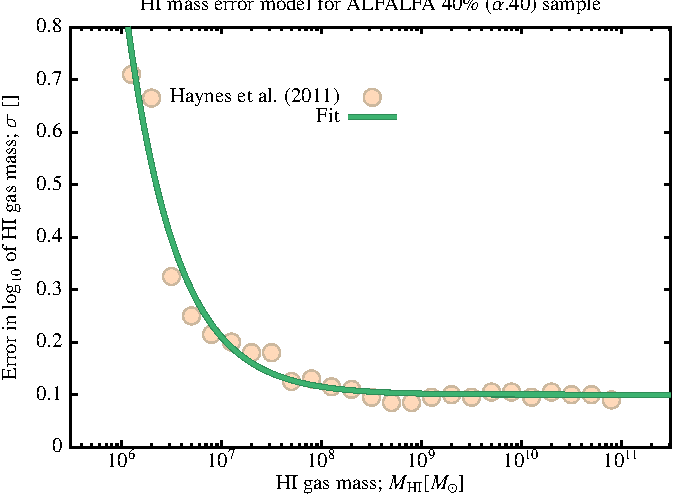
\includegraphics[width=85mm,trim=0mm 0mm 0mm 4mm,clip]{Plots/DataAnalysis/alfalfaHIMassErrorModel.pdf}
 \caption{The observational random error in galaxy HI mass as a function of HI mass for the ALFALFA survey. Points show the errors reported by \protect\cite{haynes_arecibo_2011}, while the line shows a simple functional form fit to these errors.}
 \end{center}
 \label{fig:ALFALFAErrorModel}
\end{figure}

Additionally, HI mass estimates can be affected by HI self-absorption for highly inclined galaxies. \cite[][see also \protect\citealt{zwaan_hipass_2005}]{zwaan_h_1997} estimate that this effect would lead to a mean underestimation of HI masses by a factor $1.1$ for a randomly oriented galaxy sample. Therefore, a value of $-0.0414$ for the systematic parameter {\tt [alfalfaHiMassFunctionZ0.00MassSystematic0]} is recommended.
